% $B:k6LBg3X9)3XIt>pJs%7%9%F%`9)3X2J(B
% $BB46HO@J8!&=$;NO@J8%F%s%W%l!<%H(B
%
% $BCm0U!':G?7$N%9%?%$%k%U%!%$%k$O3X2J(BWeb$B%5%$%H$K$F(B
%       $B8x3+$5$l$F$$$k$N$G!"$=$l$rI,$:3NG'$9$k$3$H(B
%
\documentclass[12pt]{jreport}
\usepackage[dvipdfmx]{graphicx} % $B?^$NE=$jIU$1MQ(B
\usepackage{ics} % ICS$BB4O@!&=$O@%9%?%$%k%U%!%$%k(B
\usepackage{makeidx} %$B:w0z@8@.MQ%Q%C%1!<%8(B
\usepackage{tabularx}% $B2#I};XDj$GI=$r:n@.(B
\usepackage{latexsym} % $B?t3X5-9fMQ%Q%C%1!<%8(B
\usepackage{url}

\newtheorem{definition}{$BDj5A(B}[chapter]
\newtheorem{algorithm}{$B%"%k%4%j%:%`(B}[chapter]

%% end of local definitions

\def\epsfsize#1#2{\ifnum#1>\hsize\hsize\else#1\fi}

\begin{document}

%$BO@J8HV9f(B
\papercode{ICS-0XM-XXX} 

% $BB46HO@J8!"=$;NO@J8$N%?%$%H%k(B
\title{$BB46HO@J8!"=$;NO@J8$N%?%$%H%k(B} 

%% $B=jB0!J3XIt!&3X2J(B or $B8&5f2J!&@l96!&%3!<%9!K(B
%\affiliation{$B9)3XIt>pJs%7%9%F%`9)3X2J(B}
%\affiliation{$B9)3XIt>pJs9)3X2J(B}
\affiliation{$BM}9)3X8&5f2J(B $B?tM}EE;R>pJs7O@l96(B\\$B>pJs%7%9%F%`9)3X%3!<%9(B}

%% $B<+J,$NL>A0!#@+$HL>$N4V$KH>3Q%9%Z!<%9$r(B1$B$D$$$l$k$3$H(B
\author{$B;a(B $BL>(B}

%% $B3X@RHV9f(B
\studentID{0XYYXXX}

%% $B3X0LO@J8$NDs=PF|(B
\date{$BNaOB(B4$BG/(B2$B7n(B10$BF|Ds=P(B}

%% $B;XF3650wL>!J@+L>!\?&0L!K(B
\supervisor{$B!{!{(B $B!y!y(B $B65<x(B}

%% $B8&5f<<$N=jB0It=p!#$h$/$o$+$i$J$$$J$i$3$N$^$^(B
\labaffiliation{$B:k6LBg3X(B $BM}9)3X8&5f2J!&9)3XIt(B}

%% $B8&5f<<L>(B
\labname{$B!{!{8&5f<<(B}

\maketitle

\setcounter{page}{1}
\chapter*{$B35MW(B}
 \pagenumbering{roman} % $B>C$5$J$$(B
 \addcontentsline{toc}{chapter}{$B35MW(B} %$B>C$5$J$$(B

 $B35MW$O!$4J7i$K$^$H$a$k$3$H!%$^$?!$O@J8$N9=@.$b35MW$N:G8e$K<($9$3$H!%(B


%%% $B<U<-(B %%%

\chapter*{$B<U<-(B}
\addcontentsline{toc}{chapter}{$B<U<-(B} % $B>C$5$J$$(B


$B8&5f$J$i$S$K@83hLL$K$*$$$F$4;XF3$$$?$@$-$^$7$?!{!{65<x$K?<$/46<U$$$?(B
$B$7$^$9!%(B

$B$^$?!$@hGZ$H$7$F$$$D$b$h$-%"%I%P%$%9$r$/$@$5$$$^$7$?!$(B
$B!{;a!$"$;a$r$O$8$a$H$9$k8&5f<<$N3'MM!$$=$7$FF14|3X@8$N3'MM!$JB$S$K;d(B
$B$rCH$+$/8+<i$C$FD:$$$?N>?F$O$8$a$H$9$k<~0O$N$9$Y$F$N3'MM$K?<$/46<U$$$?$7$^(B
$B$9!%(B

\tableofcontents % $BL\<!@8@.(B
\listoffigures % $B?^L\<!@8@.(B
\addcontentsline{toc}{chapter}{$B?^L\<!(B}
\listoftables % $BI=L\<!@8@.(B
\addcontentsline{toc}{chapter}{$BI=L\<!(B}


\chapter{$B$O$8$a$K(B} \label{chap:intro}
\pagenumbering{arabic} %$B>C$5$J$$$3$H(B
\setcounter{page}{1}   %$B>C$5$J$$$3$H(B

 \section{$BGX7J(B}
 $BGX7J(B


 \section{$BL\E*(B}
 $BL\E*(B


 \section{$BK\O@J8$N9=@.(B}
 $B9=@.!#>O$d@aHV9f$r;2>H$9$k>l9g$K$O!V(B\ref{chap:intro}$B>O$G$O!D!"(B\ref{chap:exp}$B>O$G$O!"(B\ref{sec:method}$B@a$G$O!"!W$J$I$N$h$&$K5-:\$9$k!#(B
 

\chapter{$B<B83(B} \label{chap:exp}
 \section{$B<B83J}K!(B}$B!!(B\label{sec:method}
 $B<B83J}K!(B

 \section{$B<B837k2L(B}
 $B<B837k2L(B

 
 \section{$B?^$NNc(B}

 $B4pK\E*$K$O?^$O%Z!<%8>eIt$+2<It$KCV$/$?$a%*%W%7%g%s$H$7$F$O(Bt$B$+(Bb$B$rMQ$$$k!#$^$?!"?^$N%-%c%W%7%g%s!J(Bcaption$B!K$O?^$N2<$K5-:\$9$k!#?^$NHV9f$O!V?^(B\ref{fig:reasoning_engine}$B!W$N$h$&$K;2>H$9$k!#(B
 
 \begin{figure}[tb]
 \begin{center}
  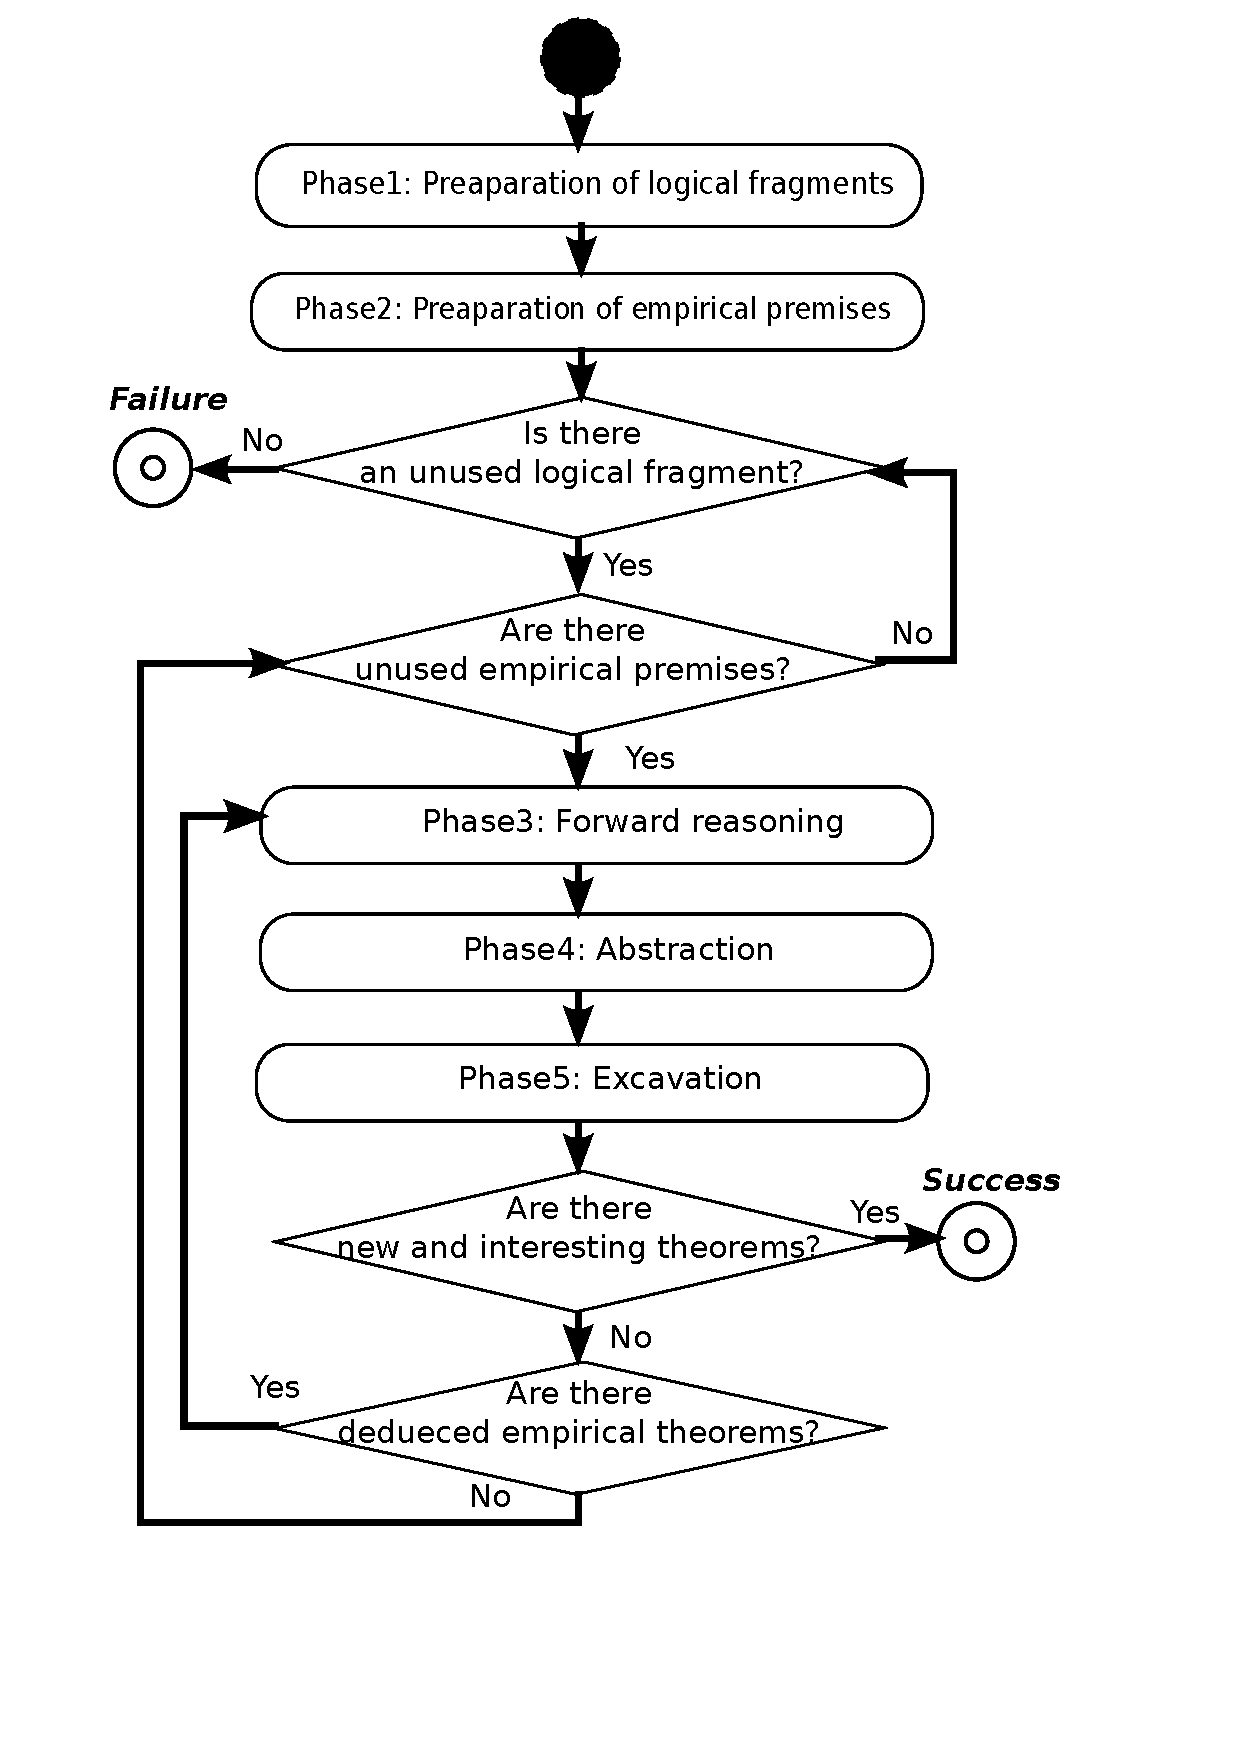
\includegraphics[scale=0.6]{fig/reasoning_engine.pdf}
  \caption{The relationship among the parts of EnCal}
  \label{fig:reasoning_engine}
 \end{center}
\end{figure}

 \section{$BI=$NNc(B}
 
 $B4pK\E*$K$OI=$O%Z!<%8>eIt$+2<It$KCV$/$?$a%*%W%7%g%s$H$7$F$O(Bt$B$+(Bb$B$rMQ$$$k!#$^$?!"I=$N%-%c%W%7%g%s!J(Bcaption$B!K$OI=$N>e$K5-:\$9$k!#I=$NHV9f$O!VI=(B\ref{tab:num_of_schemata_satisfied_srp}$B!W$N$h$&$K;2>H$9$k!#(B

$B$^$?!"I=$N7S@~$K$D$$$F$O8m2r$r>7$+$J$$$+$.$j>/$J$/$9$k$3$H$,0lHLE*$G$"$k!#:#2s$NNc$G$O!"I=8+=P$7$N2<$N7S@~$r#2=E@~$K$9$k$3$H$G8+=P$7$H%G!<%?$r8+$d$9$/J,$1$F$$$k!#$^$?!"=D$N7S@~$O:o=|$7$F$$$k!#(B
 
 \begin{table}[tb]
\begin{center}
\caption{The number of elements of $F_{k}(CML)$ and $FS_{k}(CML)$}
\label{tab:num_of_schemata_satisfied_srp}
 \begin{tabular}{c l l}
  \hline
 degree & $F_{k}(CML)$ &$FS_{k}(CML)$ \\
    & (a)&  (b)\\ 
  \hline
  \hline
  1 &  $1.60 \times 10^{1}$ & $4.00 \times 10^{0}$\\
  2 & $2.26 \times 10^{3}$ & $2.60 \times 10^{2}$  \\
  3 & $1.67 \times 10^{8}$ & $8.90 \times 10^{6}$\\
  4 & $2.92 \times 10^{19}$ & $5.15 \times 10^{17}$\\
  5 & $1.63 \times 10^{45}$ & $6.31 \times 10^{42}$\\
  6 & $4.29 \times 10^{103}$ & $2.13 \times 10^{100}$\\
  7 & $1.02 \times 10^{235}$ & $3.09 \times 10^{230}$\\
  8 & $8.15 \times 10^{527}$ & $5.61 \times 10^{521}$\\ 
  \hline
 \end{tabular}
\end{center}
\end{table}




\chapter{$B9M;!(B}
$B9M;!(B

\chapter{$B$*$o$j$K(B}
 \section{$B$^$H$a(B}
 $B$^$H$a(B

 \section{$B:#8e$N2]Bj(B}
 $B:#8e$N2]Bj(B


%%% $B=$;NO@J8$N>l9g$OI,?\!#B46HO@J8$N>l9g$OG$0U(B
\chapter*{$B8xI=O@J8(B}
\addcontentsline{toc}{chapter}{$B8xI=O@J8(B}

\begin{list}%
 {} %default label
 {} %formatting parameter
 \item $B::FIIU$-O@J8(B
       \begin{itemize}
	\item Hogehoge: ....
       \end{itemize}
 \item $B::FI$J$7O@J8(B
       \begin{itemize}
	\item Hogehoge: ....
       \end{itemize}
\end{list}
%%% $B=$;NO@J8I,?\$3$3$^$G(B %%%

\newpage

% $B;29MJ88%!'(Bbibtex$B$r;H$&>l9g(B
%
%\bibliographystyle{BST$B%U%!%$%kL>(B} % bst$B%U%!%$%kL>(B
%\bibliography{refs} % bib$B%U%!%$%kL>(B

% $B;29MJ88%!'D>@\5-=R$9$k>l9g(B
\begin{thebibliography}{99}
\label{sannkoubunnkenn_chapter}

%% $B;29MJ88%7A<0Nc(B
%
% $B$3$3$K$OG^BNJL$KJB$Y$F$$$k$,IaDL$O!"(B
% $BBh0lCx<T$N@+$NF,J8;z$G%"%k%U%!%Y%C%H=g!J(BA - Z$B!"$"!A$s!K$"$k$$$O!"(B
% $B0zMQ=g$KJB$Y$k$3$H!#$I$A$i$K$9$k$+$O;XF3650w$K3NG'$9$k$3$H!#(B

% $B@hC<>pJs%7%9%F%`9)3X8&5f<<$K$*$1$k3X0LO@J8$N;29MJ88%7A<0(B
% http://www.aise.ics.saitama-u.ac.jp/~gotoh/FormatOfReferencesInAiseLab.html

% $B3X=Q;(;oO@J8(B
% $BCx<TL>(B: $BO@J8BjL\(B, $B3X=Q;(;oL>(B, $B4,(B, $B9f(B, $B%Z!<%8?t(B, $B!J=PHG<R(B or $B=PHGCDBN!K(B, $BH/I=G/7n(B.
\bibitem{tagawa98}
$BB?@n(B $B9'1{(B, $BBgKY(B $B=gLi(B, $BDx(B $B5~FA(B, $B5mEg(B $BOBIW(B: $BAj4XO@M}$K$*$1$k6/Aj4X@-86M}(B,
        $B?M9)CNG=3X2q;o(B, Vol.\ 13, No. 3, pp.\ 387-394, 1998$BG/(B5$B7n(B.

\bibitem{Nonaka99}
Yusuke Nonaka, Jingde Cheng, and Kazuo Ushijima: A Tasking Deadlock
        Detector for Ada 95 Programs, Ada User Journal, Vol.\ 20, No.\ 1,
        pp.\ 79-92, April 1999.

% $BEE;R=PHG$N$?$a%Z!<%8?t$,3d$j?6$i$l$F$J$/!"5-;vHV9f(B1222$B$,3d$j?6$i$l$F$$$kNc!#(B
\bibitem{Sa2016}
        Inkyu Sa, Zongyuan Ge, Feras Dayoub, Ben Upcroft, Tristan Perez, and Chris McCool: DeepFruits: A Fruit Detection System Using Deep Neural Networks, Sensors Vol.\ 16 No.\ 8, e1222, August 2016.

        
% $BC19TK\(B
%  $BCx<TL>!JJT=8<T!"Lu<T!K(B: $B=qL>(B, $B=PHG<R(B or $B=PHGCDBN(B, $BH/I=G/7n(B.
\bibitem{ChengXX}
$BDx(B $B5~FA(B: $BAj4XO@M}F~Lg(B, $B2?$i$+=PHG<R(B, 200?$BG/(B?$B7n(B.

\bibitem{Jin01}
Qun Jin, Jie LI, Nan Zhang, Jingde Cheng, Clement Yu, and Shoichi
        Noguchi: Enabling Society with Information Technology,
        Springer-Verlag, November 2001.

% $BK]LuK\$N>l9g$O86Cx$N>pJs$N8e$KK]LuK\$N>pJs$r=q$/(B
\bibitem{Hennessy93}
Matthew Hennessy: The Semantics of Programming Languages, John Wiley and
Sons, Ltd., 1990. ($B%^%7%e!<(B $B%X%M%7!<Cx(B, $B9SLZ(B $B7<FsO:(B, $BDx(B $B5~FA(B $B6&Lu(B: $B%W%m(B
$B%0%i%_%s%08@8l$N0UL#O@F~Lg(B, $B%5%$%(%s%9<R(B, 1993$BG/(B.)

% $B9q:]2q5D!"9qFb%7%s%]%8%&%`O@J8=8O@J8(B
% $BCx<TL>(B: $BO@J8BjL\(B, $B2q5DL>!\2q5DN,>N(B, $B%Z!<%8?t(B, $B2q5D3+:ECO(B, $B2q5D3+:E9q(B,$B!J=PHG<R(B or $B=PHGCDBN!K(B, $BH/I=G/7n(B.
\bibitem{Goto01}
Yuichi Goto, Daisuke Takahashi, and Jingde Cheng: Parallel Forward
        Deduction Algorithms of General-Purpose Entailment Calculus on
        Shared-Memory Parallel Computers, Proceedings of the ACIS 2nd
        International Conference on Software Engineering, Artificial
        Intelligence, Networking \& Parallel/Distributed Computing,
        pp.\ 168-175, Nagoya, Japan, August 2001.

\bibitem{Koide01}
$B>.=P(B $B2m?M(B, $BDx(B $B5~FA(B: $B%$%s%?!<%M%C%H>e$G%+!<%I%2!<%`$r9T$&$?$a$NHFMQ%W%m%H(B
        $B%3%k72$N3+H/(B, $B>pJs=hM}3X2qBh#62s%2!<%`!&%W%m%0%i%_%s%09q:]%o!<%/(B
        $B%7%g%C%WO@J8=8(B, pp.\ 78-85, $BH":,(B, $BF|K\(B, 2001 $BG/(B10$B7n(B.

% $BO@J8=8%7%j!<%:$dC19TK\$K<}O?$5$l$?O@J8(B
% $BCx<TL>(B: $BO@J8BjL\(B, $BJT=8<T!J(Beditor$B!K(B, $B=qL>(B, $BO@J8=8%7%j!<%:L>(B, $BO@J8=8%7%j!<%:4,?t(B, $B%Z!<%8?t(B, $B=PHG<R(B or $B=PHGCDBN(B, $BH/I=G/7n(B.
\bibitem{Cheng91}
Jingde Cheng: Relevance Logic and Entailment Logic, in I.\ Nakada and
        M.\ Hagiya (Eds.), ``Software Science and Engineering,''
        pp.\ 189-211, World Scientific, November 1991.

\bibitem{Nonaka00}
Yusuke Nonaka, Jingde Cheng, and Kazuo Ushijima: A Supporting Tool for
        Development of Self-measurement Ada Programs, in H.\ B.\ Keller
        and E.\ Ploedereder (Eds.), ``Reliable Software Technologies -
        Ada-Europe 2000, 5th International Conference on Reliable
        Software Technologies, Potsdam, Germany, June 2000,
        Proceedings,'' Lecture Notes in Computer Science, Vol.\ 1845,
        pp.\ 69-81, Springer-Verlag, June 2000.


% $BGn;N!$=$;N!$B46HO@J8(B
\bibitem{Goto05}
$B8eF#(B $BM40l(B: $B6/Aj4XO@M}$K4p$E$$$?<+F0A08~$-1ieh$H$=$N1~MQ(B, $B:k6LBg3XBg3X1!(B
	$BM}9)3X8&5f2J>pJs?tM}2J3X@l96Gn;NO@J8(B, 2005$BG/(B3$B7n(B.

\bibitem{Goto02}
$B8eF#(B $BM40l(B: $B6/Aj4XO@M}$HHFMQA08~$-<+F05"7k1i;;%7%9%F%`(B EnCal $B$rMQ$$$?CN<1(B
	$BH/8+(B, $B:k6LBg3XBg3X1!M}9)3X8&5f2J>pJs%7%9%F%`9)3X@l96=$;NO@J8(B, 2003$BG/(B
	2$B7n(B.

\bibitem{Goto00}
$B8eF#(B $BM40l(B: $BHFMQA08~$-<+F05"7k1i;;%7%9%F%`(BEnCal$B$N6&M-%a%b%j7?JBNs7W;;5!>e(B
	$B$G$NJBNs2=(B, $B:k6LBg3X9)3XIt>pJs%7%9%F%`9)3X2JB46HO@J8(B, 2001$BG/(B2$B7n(B.


% $B4k6H$d@=IJ$N(BWeb$B%Z!<%8$J$I(B
% \newblock$B$O8e$m$KB3$/J8;zNs$r0l$D$N2t$H$7$F$_$J$9L?Na(B
\bibitem{cem}
Common Criteria Project: CEM v3.1,
\url{http://www.commoncriteriaportal.org/thecc.html}
(accessed 2007-04-05).

\bibitem{ipsjweb}
$B>pJs=hM}3X2q(B: $B%3%s%T%e!<%?GnJ*4[@_N)$NDs8@(B, \url{http://www.ipsj.or.jp/03somu/teigen/museum200702.html} ($B;2>H(B2007-02-05).

\end{thebibliography}

% $BIUO?(B
\appendix % $B0J2<!$IUO?(B
\chapter{$B"&"$"&"$(B}
\section{$B$[$2$[$2(B}
\section{$B$[$j$c$[$j$c(B}
\chapter{$B"&"$"&"$(B}
\section{$B$[$2$[$2(B}
\section{$B$[$j$c$[$j$c(B}

% $B:w0z$r$D$1$k>l9g$K$O(B
% mendex$B$+(Bmkindex$B$G:n@.(B
%\printindex

%$BL\<!$K(BIndex$B$rI=<($5$;$k>l9g$O(Bmendex$B$+(Bmkindex$B<B9T8e$K:n@.$5$l$k(B
% hogehoge.idm$B%U%!%$%k$N(Btheindex$B4D6-$NCf$G2<5-L?Na$rCV$/(B
%\addcontentsline{toc}{chapter}{Index}

\end{document}

